% University of Udine Assignment Template
% Based on the unofficial University of Udine beamer template
% Adapted for assignment/homework document format

\documentclass[tikz,12pt,a4paper]{article}

%%% Packages
\usepackage[utf8]{inputenc}
\usepackage[margin=2.5cm]{geometry}
\usepackage{graphicx}
\usepackage{amsmath,amssymb,amsthm}
\usepackage{xcolor}
\usepackage{titlesec}
\usepackage{fancyhdr}
\usepackage{enumitem}
\usepackage{tcolorbox}
\usepackage{hyperref}

\usepackage{tikz}
\usetikzlibrary{positioning,arrows.meta}


%%% University of Udine Colors
% These colors are defined following the "Manuale di Stile"
% (Style Manual) of the University of Udine
\definecolor{UniOrange}{RGB}{242,140,41}
\definecolor{UniBlue}{RGB}{51,102,153}
\definecolor{UniBrown}{RGB}{102,51,0}
\definecolor{UniGold}{RGB}{204,153,0}

%%% Hyperref setup
\hypersetup{
    colorlinks=true,
    linkcolor=UniBlue,
    urlcolor=UniBlue,
    citecolor=UniBlue,
}

%%% Header and Footer
\pagestyle{fancy}
\fancyhf{}
\fancyhead[L]{\textcolor{UniBrown}{\assignmentcode}}
\fancyhead[R]{\textcolor{UniBrown}{\shortauthor}}
\fancyfoot[C]{\textcolor{UniBrown}{\thepage}}
\renewcommand{\headrulewidth}{0.5pt}
\renewcommand{\footrulewidth}{0pt}
\renewcommand{\headrule}{\hbox to\headwidth{\color{UniOrange}\leaders\hrule height \headrulewidth\hfill}}

%%% Section formatting
\titleformat{\section}
  {\Large\bfseries\color{UniOrange}}
  {\thesection}{1em}{}
  [\titlerule]

\titleformat{\subsection}
  {\large\bfseries\color{UniBrown}}
  {\thesubsection}{1em}{}

\titleformat{\subsubsection}
  {\normalsize\bfseries\color{UniBrown}}
  {\thesubsubsection}{1em}{}

%%% Custom commands
\newcommand{\marker}[2][UniOrange]{\colorbox{#1!30}{#2}}

%%% Custom boxes using tcolorbox
\tcbuselibrary{skins,breakable}

% Question box
\newtcolorbox{questionbox}[1][]{
  colback=UniOrange!5,
  colframe=UniOrange,
  fonttitle=\bfseries,
  title={Question},
  breakable,
  #1
}

% Solution box
\newtcolorbox{solutionbox}[1][]{
  colback=UniBlue!5,
  colframe=UniBlue,
  fonttitle=\bfseries,
  title={Solution},
  breakable,
  #1
}

% Note box
\newtcolorbox{notebox}[1][]{
  colback=UniGold!10,
  colframe=UniGold,
  fonttitle=\bfseries,
  title={Note},
  breakable,
  #1
}

% Important box
\newtcolorbox{importantbox}[1][]{
  colback=UniBrown!5,
  colframe=UniBrown,
  fonttitle=\bfseries,
  title={Important},
  breakable,
  #1
}

%%% Theorem environments
\theoremstyle{definition}
\newtheorem{definition}{Definition}[section]
\newtheorem{theorem}{Theorem}[section]
\newtheorem{lemma}[theorem]{Lemma}
\newtheorem{proposition}[theorem]{Proposition}
\newtheorem{corollary}[theorem]{Corollary}
\newtheorem{example}{Example}[section]

%%% Itemize styling
\setlist[itemize,1]{label=\textcolor{UniOrange}{$\bullet$}}
\setlist[itemize,2]{label=\textcolor{UniBrown}{$\circ$}}
\setlist[enumerate,1]{label=\textcolor{UniOrange}{\arabic*.}}
\setlist[enumerate,2]{label=\textcolor{UniBrown}{\alph*)}}

%%% Title page information
\newcommand{\assignmentcode}{Assignment Code}
\newcommand{\assignmenttitle}{Assignment Title}
\newcommand{\assignmentdate}{\today}
\newcommand{\coursename}{Course Name}
\newcommand{\studentname}{Student Name}
\newcommand{\studentid}{Student ID}
\newcommand{\shortauthor}{Student Name}

%%% Custom title page
\newcommand{\maketitlepage}{
  \begin{titlepage}
    \centering
    \vspace*{2cm}
    
    % University Logo (uncomment and adjust path if you have a logo)
    % \includegraphics[width=0.3\textwidth]{logo_uniud.png}\\[1cm]
    
    {\Large \textcolor{UniBrown}{\textbf{University of Udine}}}\\[0.5cm]
    {\large \textcolor{UniBrown}{DMIF}}\\[2cm]
    
    {\huge \textcolor{UniOrange}{\textbf{\assignmentcode}}}\\[0.5cm]
    {\Large \textcolor{UniBrown}{\assignmenttitle}}\\[1.5cm]
    
    {\large \textcolor{UniBrown}{\coursename}}\\[2cm]
    
    \begin{minipage}{0.4\textwidth}
      \begin{flushleft}
        \textcolor{UniBrown}{\textbf{Student:}}\\
        \studentname\\
        ID: \studentid
      \end{flushleft}
    \end{minipage}
    \hfill
    \begin{minipage}{0.4\textwidth}
      \begin{flushright}
        \textcolor{UniBrown}{\textbf{Date:}}\\
        \assignmentdate
      \end{flushright}
    \end{minipage}
    
    \vfill
  \end{titlepage}
}

%%% Bibliography (if needed)
\usepackage[style=authoryear,backend=biber]{biblatex}
% \addbibresource{references.bib}  % Uncomment and add your .bib file

%%%%%%%%%%%%%%%%%%%%%%%%%%%%%%%%%%%%%%%%%%%%%%%%%%%%%%%%%
%%% DOCUMENT INFORMATION - CUSTOMIZE THESE
%%%%%%%%%%%%%%%%%%%%%%%%%%%%%%%%%%%%%%%%%%%%%%%%%%%%%%%%%

\renewcommand{\assignmentcode}{Foundations Of Neural Networks}
\renewcommand{\assignmenttitle}{Connect-4 as a Testbed: Analyzing Learning Trajectories in a Solved Game}
\renewcommand{\assignmentdate}{October 22, 2025}
\renewcommand{\coursename}{Foundations Of Neural Networks}
\renewcommand{\studentname}{Luca Simonetti}
\renewcommand{\studentid}{172161}
\renewcommand{\shortauthor}{L. Simonetti}

%%%%%%%%%%%%%%%%%%%%%%%%%%%%%%%%%%%%%%%%%%%%%%%%%%%%%%%%%

\begin{document}

%%% Title Page
\maketitlepage

%%% Table of Contents (optional)
\tableofcontents
\newpage

%%%%%%%%%%%%%%%%%%%%%%%%%%%%%%%%%%%%%%%%%%%%%%%%%%%%%%%%%
%%% ASSIGNMENT CONTENT STARTS HERE
%%%%%%%%%%%%%%%%%%%%%%%%%%%%%%%%%%%%%%%%%%%%%%%%%%%%%%%%%

\section{Introduction}

Connect-4 is a solved game—its outcome under perfect play from any position has been known since 1988, when James D. Allen first proved the first player can force a win, with Victor Allis providing a complete solution in 1988. In game theory, a solved game is one whose outcome (win, loss, or draw) can be correctly predicted from any position when both players employ optimal strategies. This property makes Connect-4 an ideal testbed for machine learning research: we can evaluate how well learning algorithms discover known optimal strategies and understand the mechanisms by which they do so.

This report investigates how neural networks learn to play Connect-4 from a super-expert teacher, focusing on three key questions:
\begin{itemize}
    \item How does network architecture size affect learning dynamics and final performance?
    \item How does the weight space evolve during training, and what does this reveal about the optimization landscape?
    \item How does the learned representation space develop, and what features emerge to support strategic play?
\end{itemize}

By analyzing these aspects, we aim to gain insights into both the specific problem of game-playing agents and the broader question of how neural networks learn structured, strategic reasoning.

\section{Related Work}

\section{Method}
Neural networks are notoriously hard to decipher and intrinsically opaque. In order to make sense of their learning dynamics, a key assumption is made: since Connect-4 is a solved game, we can use a perfect player as a teacher to provide supervision. This allows us to focus on how the network learns to approximate this optimal strategy rather than discovering it from scratch.
It needs to be kept in mind that MCTS follows a very precise pipeline dividing into a tree search phase followed by a move selection phase. The tree search phase is responsible for exploring the game tree and gathering statistics about the possible moves, while the move selection phase uses these statistics to choose the best move to play. In this work, we focus on training neural networks to mimic the move selection phase of a perfect MCTS player.

In other words, given a board state, the network is trained to predict the policy (i.e., the probability distribution over possible moves) and value (i.e., the expected outcome of the game from that state) outputs of the MCTS player. This setup allows to analyze how well different network architectures can learn to approximate the optimal strategy provided by the MCTS teacher.

It can be easily measure how well the network learns epoch by epoch by evaluating its performance against the MCTS player on a validation set of board states. This provides a clear metric for assessing learning progress and final performance.

With this setup, it is possible to systematically vary the network architecture size (e.g., number of layers, number of neurons per layer) and analyze how these changes impact learning dynamics, weight space evolution, and representation development.

\subsection{Experiment Setup}
It's employed an existing implementation of an AlphaZero-like MCTS player for Connect-4 as teacher. The neural networks are trained using supervised learning to predict the MCTS player's policy and value outputs given board states. 
This is done by first creating a dataset of board states representing various game situations, along with the corresponding policy and value outputs from the MCTS player. The networks are then trained on this dataset using standard optimization techniques (i.e., stochastic gradient descent) and loss functions (e.g., cross-entropy for policy, mean squared error for value).

This dataset is then split into training and validation sets to monitor learning progress and prevent overfitting. The networks are evaluated on the validation set after each epoch to track performance improvements.


\subsection{Architecture}
  The proposed architecture follows a two-stage design that combines convolutional and recurrent components. The first stage employs a residual convolutional block inspired by ResNet architecture, consisting of
  two sequential layers, each comprising a convolutional layer followed by batch normalization and ReLU activation. This can be expressed as:
  \[
  (\mathrm{Conv} \rightarrow \mathrm{BatchNorm} \rightarrow \mathrm{ReLU}) \times 2.
  \]

  The convolutional stage is followed by a recurrent module implemented using Gated Recurrent Units (GRUs), which capture temporal dependencies in the processed features. The key idea is to separate the planning
  responsibilities into two complementary high-dimensional representations:
  \begin{itemize}
      \item \textbf{Spatial:} the CNN must produce an expressive embedding of the current board configuration irrespective of past moves; the same CNN weights are reused at every timestep.
      \item \textbf{Temporal:} the GRU ingests the entire sequence of CNN embeddings \(z_{1:T}\), maintaining an internal state \(h_t\) that integrates match history and informs future decisions.
  \end{itemize}

  \begin{figure}[ht]
    \centering
    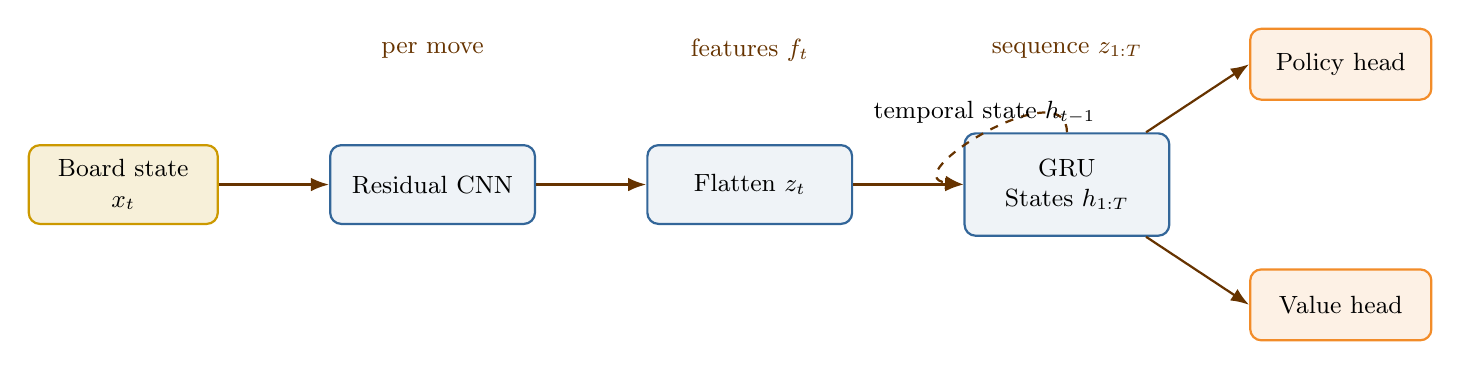
\begin{tikzpicture}[font=\small, >=Latex, node distance=1.4cm]
      \tikzset{
        tensor/.style={draw=UniGold, thick, rounded corners, minimum width=2.4cm, minimum height=1.0cm, align=center, fill=UniGold!15},
        block/.style={draw=UniBlue, thick, rounded corners, minimum width=2.6cm, minimum height=1.0cm, align=center, fill=UniBlue!8},
        head/.style={draw=UniOrange, thick, rounded corners, minimum width=2.3cm, minimum height=0.9cm, align=center, fill=UniOrange!12},
        arrow/.style={->, thick, draw=UniBrown}
      }
      \node[tensor] (input) {Board state\\$x_t$};
      \node[block, right=of input] (cnn) {Residual CNN};
      \node[block, right=of cnn] (flatten) {Flatten $z_t$};
      \node[block, right=of flatten, minimum height=1.3cm] (gru) {GRU\\States $h_{1:T}$};
      \node[head, above right=0.4cm and 1.0cm of gru] (policy) {Policy head};
      \node[head, below right=0.4cm and 1.0cm of gru] (value) {Value head};

      \draw[arrow] (input) -- (cnn);
      \draw[arrow] (cnn) -- (flatten);
      \draw[arrow] (flatten) -- (gru);
      \draw[arrow] (gru) -- (policy.west);
      \draw[arrow] (gru) -- (value.west);
      \draw[arrow, dashed] (gru.north) .. controls +(0,0.8) and +(-0.9,0.1) .. node[pos=0.52, above, align=center]{temporal state $h_{t-1}$} (gru.west);

      \node[above of=cnn, yshift=0.3cm, text=UniBrown] {per move};
      \node[above of=flatten, yshift=0.3cm, text=UniBrown] {features $f_t$};
      \node[above of=gru, yshift=0.3cm, text=UniBrown] {sequence $z_{1:T}$};
    \end{tikzpicture}
    \caption{Two-stage architecture: the CNN maps each board to a spatial embedding, while the GRU integrates the move sequence before producing policy and value predictions.}
  \end{figure}

  After the GRU, two task-specific heads operate on each hidden state: a policy head that outputs logits over the seven columns, and a value head that predicts the expected outcome. This design ensures the CNN is invoked before every move to model spatial structure at time \(t\), while the GRU observes the whole trajectory and communicates its training signal back to the CNN through backpropagation.
More formally:
  Let $x_t \in \mathbb{R}^{3 \times 6 \times 7}$ denote the Connect-4 board at move $t$, $t = 1,\dots,T$.
  The CNN feature extractor with parameters $\theta_c$ produces spatial embeddings
  \begin{align}
      f_t &= \operatorname{CNN}_{\theta_c}(x_t) \in \mathbb{R}^{C \times 6 \times 7},\\
      z_t &= \operatorname{vec}(f_t) \in \mathbb{R}^{C \cdot 6 \cdot 7}.
  \end{align}

  The GRU with parameters $\theta_g = \{W_r,U_r,b_r,W_u,U_u,b_u,W_h,U_h,b_h\}$ consumes the entire sequence $z_{1:T}$:
  \begin{align}
      r_t &= \sigma(W_r z_t + U_r h_{t-1} + b_r),\\
      u_t &= \sigma(W_u z_t + U_u h_{t-1} + b_u),\\
      \tilde{h}_t &= \tanh\!\big(W_h z_t + U_h (r_t \odot h_{t-1}) + b_h\big),\\
      h_t &= (1-u_t) \odot h_{t-1} + u_t \odot \tilde{h}_t, \qquad h_0 = 0.
  \end{align}

  Policy and value heads with parameters $\theta_p,\theta_v$ act on each $h_t$:
  \begin{align}
      \pi_t &= W_p h_t + b_p, \\
      v_t &= \tanh\!\big(W_v^{(2)} \operatorname{ReLU}(W_v^{(1)} h_t + b_v^{(1)}) + b_v^{(2)}\big).
  \end{align}

  Given ground-truth move labels $y_t$ and returns $r_t^{\text{target}}$, the loss aggregates over the sequence,
  \begin{equation}
      \mathcal{L} = \sum_{t=1}^{T} \left(
          \mathcal{L}_{\text{policy}}(\pi_t, y_t) +
          \lambda \,\mathcal{L}_{\text{value}}(v_t, r_t^{\text{target}})
      \right),
  \end{equation}
  with balancing coefficient $\lambda$.

  \subsection*{Backward Pass (BPTT)}

  Initialize $g_{T+1}^{(h)} = 0$ and propagate backwards:
  \begin{equation}
      g_t^{(h)} = \frac{\partial \mathcal{L}_{\text{policy},t}}{\partial h_t}
                + \frac{\partial \mathcal{L}_{\text{value},t}}{\partial h_t}
                + \left(\frac{\partial h_{t+1}}{\partial h_t}\right)^{\!\top} g_{t+1}^{(h)}.
  \end{equation}
  For the GRU,
  \begin{align}
      g_t^{(\tilde{h})} &= g_t^{(h)} \odot u_t \odot (1 - \tilde{h}_t^2),\\
      g_t^{(u)} &= g_t^{(h)} \odot (\tilde{h}_t - h_{t-1}),\\
      g_t^{(r)} &= \big(U_h^\top g_t^{(\tilde{h})} \odot h_{t-1}\big) \odot r_t \odot (1 - r_t),\\
      g_t^{(z)} &= W_r^\top g_t^{(r)} + W_u^\top g_t^{(u)} + W_h^\top g_t^{(\tilde{h})}.
  \end{align}
  Gradients w.r.t.\ the GRU parameters follow the usual outer-product forms, e.g.\ $\partial \mathcal{L}/\partial W_r = \sum_t g_t^{(r)} z_t^\top$, etc.

  Finally, the gradient reaching the CNN at each timestep is
  \begin{equation}
      \frac{\partial \mathcal{L}}{\partial \theta_c}
      = \sum_{t=1}^{T}
          \left( \frac{\partial f_t}{\partial \theta_c} \right)^{\!\top}
          \operatorname{reshape}\!\left( g_t^{(z)} \right),
  \end{equation}
  so the CNN receives full BPTT signal via every $z_t$ while the GRU captures the temporal dependencies across the match.
  \begin{notebox}
  Intuitively, the key idea is that the GRU’s backward signal should tell the CNN which features in its embeddings must change to reduce $\mathcal{L}$, effectively communicating "what it needs" from each spatial representation in order to improve performance.
  \end{notebox}
  

\subsection{Question Box}

\begin{questionbox}
Prove that the sum of two even numbers is always even.
\end{questionbox}

\subsection{Solution Box}

\begin{solutionbox}
Let $a = 2m$ and $b = 2n$ where $m, n \in \mathbb{Z}$. Then:
\begin{equation}
a + b = 2m + 2n = 2(m + n)
\end{equation}
Since $(m + n) \in \mathbb{Z}$, the sum $a + b$ is even.
\end{solutionbox}

\subsection{Note Box}

\begin{notebox}
This proof uses the definition of even numbers: a number is even if it can be expressed as $2k$ for some integer $k$.
\end{notebox}

\subsection{Important Box}

\begin{importantbox}
Remember to show all your work and justify each step in your solutions.
\end{importantbox}

\section{Mathematical Environments}

\begin{definition}[Even Number]
An integer $n$ is \textbf{even} if there exists an integer $k$ such that $n = 2k$.
\end{definition}

\begin{theorem}[Fundamental Theorem]
This is an example of a theorem environment.
\end{theorem}

\begin{example}
The number 6 is even because $6 = 2 \cdot 3$.
\end{example}

\section{Lists and Enumerations}

\subsection{Itemized List}

The following are properties of even numbers:
\begin{itemize}
  \item The sum of two even numbers is even
  \item The product of two even numbers is even
  \item The difference of two even numbers is even
  \begin{itemize}
    \item This is a nested item
    \item Another nested item
  \end{itemize}
\end{itemize}

\subsection{Enumerated List}

To solve this problem, follow these steps:
\begin{enumerate}
  \item Read the question carefully
  \item Identify the given information
  \item Apply the appropriate theorem or formula
  \begin{enumerate}
    \item This is a sub-step
    \item Another sub-step
  \end{enumerate}
  \item Write your final answer
\end{enumerate}

\section{Text Highlighting}

You can use the \textbackslash marker command to \marker{highlight important text} or use \marker[UniBlue]{different colors} like \marker[UniBrown]{brown} or \marker[UniGold]{gold}.

\section{Exercises}

\begin{questionbox}[title={Exercise 1}]
Calculate the derivative of $f(x) = x^3 + 2x^2 - 5x + 1$.
\end{questionbox}

\begin{solutionbox}[title={Solution to Exercise 1}]
Using the power rule:
\begin{align}
f'(x) &= \frac{d}{dx}(x^3 + 2x^2 - 5x + 1) \\
      &= 3x^2 + 4x - 5
\end{align}
\end{solutionbox}

\begin{questionbox}[title={Exercise 2}]
Evaluate the integral $\displaystyle\int_0^1 x^2 \, dx$.
\end{questionbox}

\begin{solutionbox}[title={Solution to Exercise 2}]
\begin{align}
\int_0^1 x^2 \, dx &= \left[\frac{x^3}{3}\right]_0^1 \\
                    &= \frac{1^3}{3} - \frac{0^3}{3} \\
                    &= \frac{1}{3}
\end{align}
\end{solutionbox}

\section{Conclusion}

This template provides a clean and professional format for your assignments while maintaining the visual identity of the University of Udine.

%%%%%%%%%%%%%%%%%%%%%%%%%%%%%%%%%%%%%%%%%%%%%%%%%%%%%%%%%
%%% BIBLIOGRAPHY (if needed)
%%%%%%%%%%%%%%%%%%%%%%%%%%%%%%%%%%%%%%%%%%%%%%%%%%%%%%%%%

% \newpage
% \printbibliography

\end{document}
